\section{Data Warehouse Modeling: Data Cube and OLAP}

% TODO: Example ERM for sales

\begin{frame}{From Tables and Spreadsheets to Data Cubes}
	\begin{itemize}
		\item Data warehouse:
		      \begin{itemize}
			      \item Based on a \textbf{\color{airforceblue}multidimensional data model} which views data in the form of a \textbf{data cube}.
		      \end{itemize}
		\item \textbf{Data cube.}
		      \begin{itemize}
			      \item Allows data (here: sales) to be modeled and viewed in multiple dimensions.
			            \begin{itemize}
				            \item \textbf{Dimension tables:} such as: \texttt{item (item\_name, brand, type)},\\
				                  or: \texttt{time (day, week, month, quarter, year)}.
				            \item \textbf{Fact table:} Contains \textbf{measures} (such as \texttt{dollars\_sold}) and references (\texttt{foreign keys}) to each of the related dimension tables.
			            \end{itemize}
		      \end{itemize}
		\item \textbf{$n$-dimensional base cube.}
		      \begin{itemize}
			      \item Called a base cuboid in data warehousing literature.
		      \end{itemize}
		\item \textbf{Top most $0$-dimensional cuboid.}
		      \begin{itemize}
			      \item Holds the highest-level of summarization.
			      \item Called the apex cuboid.
		      \end{itemize}
		\item \textbf{Lattice of cuboids.} (Forms a data cube)
	\end{itemize}
\end{frame}

\begin{frame}{Cube: A Lattice of Cuboids}
	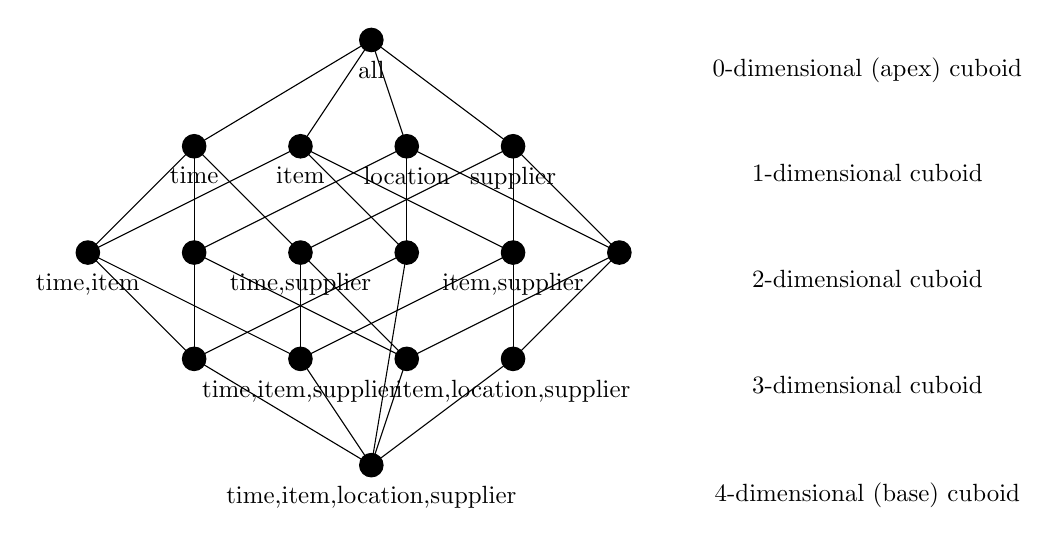
\begin{tikzpicture}[
			scale=0.9,
			every node/.style={transform shape},
		]
		\node[draw, circle, fill=black, label=below:{all}] at (2,6) {};
		\draw (2,6) -- (-0.5,4.5);
		\draw (2,6) -- (1,4.5);
		\draw (2,6) -- (2.5,4.5);
		\draw (2,6) -- (4,4.5);

		\node[draw, circle, fill=black, label=below:{time}] at (-0.5,4.5) {};
		\node[draw, circle, fill=black, label=below:{item}] at (1,4.5) {};
		\node[draw, circle, fill=black, label=below:{location}] at (2.5,4.5) {};
		\node[draw, circle, fill=black, label=below:{supplier}] at (4,4.5) {};

		\draw (-0.5,4.5) -- (-2,3);
		\draw (-0.5,4.5) -- (-0.5,3);
		\draw (-0.5,4.5) -- (1,3);
		\draw (1,4.5) -- (-2,3);
		\draw (1,4.5) -- (2.5,3);
		\draw (1,4.5) -- (4,3);
		\draw (2.5,4.5) -- (-0.5,3);
		\draw (2.5,4.5) -- (2.5,3);
		\draw (2.5,4.5) -- (5.5,3);
		\draw (4,4.5) -- (1,3);
		\draw (4,4.5) -- (4,3);
		\draw (4,4.5) -- (5.5,3);


		\node[draw, circle, fill=black, label=below:{time,item}] at (-2,3) {};
		\node[draw, circle, fill=black] at (-0.5,3) {};
		\node[draw, circle, fill=black, label=below:{time,supplier}] at (1,3) {};
		\node[draw, circle, fill=black] at (2.5,3) {};
		\node[draw, circle, fill=black, label=below:{item,supplier}] at (4,3) {};
		\node[draw, circle, fill=black] at (5.5,3) {};
		\draw (-2,3) -- (-0.5,1.5);
		\draw (-2,3) -- (1,1.5);
		\draw (-0.5,3) -- (-0.5,1.5);
		\draw (-0.5,3) -- (2.5,1.5);
		\draw (1,3) -- (1,1.5);
		\draw (1,3) -- (2.5,1.5);
		\draw (2.5,3) -- (-0.5,1.5);
		\draw (2.5,3) -- (2,0);
		\draw (4,3) -- (1,1.5);
		\draw (4,3) -- (4,1.5);
		\draw (5.5,3) -- (2.5,1.5);
		\draw (5.5,3) -- (4,1.5);

		\node[draw, circle, fill=black] at (-0.5,1.5) {};
		\node[draw, circle, fill=black, label=below:{time,item,supplier}] at (1,1.5) {};
		\node[draw, circle, fill=black] at (2.5,1.5) {};
		\node[draw, circle, fill=black, label=below:{item,location,supplier}] at (4,1.5) {};
		\draw (-0.5,1.5) -- (2,0);
		\draw (1,1.5) -- (2,0);
		\draw (2.5,1.5) -- (2,0);
		\draw (4,1.5) -- (2,0);

		\node[draw, circle, fill=black, label=below:{time,item,location,supplier}] at (2,0)  {};

		\node[label=below:{$0$-dimensional (apex) cuboid}] at (9,6)  {};
		\node[label=below:{$1$-dimensional cuboid}] at (9,4.5)  {};
		\node[label=below:{$2$-dimensional cuboid}] at (9,3)  {};
		\node[label=below:{$3$-dimensional cuboid}] at (9,1.5)  {};
		\node[label=below:{$4$-dimensional (base) cuboid}] at (9,0)  {};
	\end{tikzpicture}
\end{frame}

\begin{frame}{Conceptual Modeling of Data Warehouses}
	\begin{enumerate}
		\item \textbf{Star schema:}.
		      \begin{itemize}
			      \item A fact table in the middle connected to a set of dimension tables.
		      \end{itemize}
		\item \textbf{Snowflake schema:}.
		      \begin{itemize}
			      \item A refinement of the star schema where some dimensional hierarchies \\
			            are \textbf{normalized} into a set of smaller dimension tables,\\
			            forming a shape similar to a snowflake.
			      \item I. e. dimension tables of a star schema are split into multiple (dimension) tables\\ along their respective granularity level, but not split/normalized for every granularity.
		      \end{itemize}
		\item \textbf{Fact constellations:}.
		      \begin{itemize}
			      \item Multiple fact tables sharing dimension tables, \\
			            viewed as a collection of stars, therefore called \\
			            \textbf{galaxy schema} or fact constellation.
		      \end{itemize}
	\end{enumerate}
\end{frame}

\begin{frame}{Example of a Star Schema}
	\begin{tikzpicture}
		\node[basic, rectangle split part fill={green!20,white}] at (2,2) (time) {time
			\nodepart{second}
			\underline{time\_key}\\
			day\\
			day\_of\_week\\
			month\\
			quarter\\
			year};

		\node[basic] at (2,-1.5) (branch) {branch
			\nodepart{second}
			\underline{branch\_key}\\
			branch\_name\\
			branch\_type};

		\node[basic, rectangle split part fill={orange!20,white}] at (12,2) (item) {item
			\nodepart{second}
			\underline{item\_key}\\
			item\_name\\
			brand\\
			type\\
			supplier\_type};

		\node[basic, rectangle split part fill={yellow!20,white}] at (12,-1.25) (location) {location
			\nodepart{second}
			\underline{location\_key}\\
			street\\
			city\\
			province\\
			country};

		\node[] at (7,3) {Sales fact table:};
		\node[fill=green!20, minimum width = 3cm, minimum height=0.5cm, align=right] at (7,2.5) (a) {time\_key};
		\node[fill=orange!20, minimum width = 3cm, minimum height=0.5cm, align=right] at (7,2) (b) {item\_key};
		\node[fill=blue!20, minimum width = 3cm, minimum height=0.5cm, align=right] at (7,1.5) (c) {branch\_key};
		\node[fill=yellow!20, minimum width = 3cm, minimum height=0.5cm, align=right] at (7,1) (d) {location\_key};
		\node[fill=red!20, minimum width = 3cm, minimum height=0.5cm, align=right] at (7,0.5) (units) {units\_sold};
		\node[fill=red!20, minimum width = 3cm, minimum height=0.5cm, align=right] at (7,0) (dollars) {dollars\_sold};
		\node[fill=red!20, minimum width = 3cm, minimum height=0.5cm, align=right] at (7,-0.5) (sales) {avg\_sales};
		\draw[->, dashed] (a.west) -- (time);
		\draw[->, dashed] (b) -- (item);
		\draw[->, dashed] (c.west) -- (branch);
		\draw[->, dashed] (d.east) -- (location);

		\node[fill=red!20, minimum width = 3cm, minimum height=0.5cm, align=right] at (5,-1.5) (e) {Measures};
		\draw[-] (e) -- (units.west);
		\draw[-] (e) -- (dollars.west);
		\draw[-] (e) -- (sales.west);
	\end{tikzpicture}
\end{frame}

\begin{frame}{Example of Snowflake Schema}
	\begin{tikzpicture}
		\node[basic, rectangle split part fill={green!20,white}] at (2,2) (time) {time
			\nodepart{second}
			\underline{time\_key}\\
			day\\
			day\_of\_week\\
			month\\
			quarter\\
			year};

		\node[basic] at (2,-1.5) (branch) {branch
			\nodepart{second}
			\underline{branch\_key}\\
			branch\_name\\
			branch\_type};

		\node[basic, rectangle split part fill={orange!20,white}] at (10,2) (item) {item
			\nodepart{second}
			\underline{item\_key}\\
			item\_name\\
			brand\\
			type\\
			supplier\_key};

		\node[basic, rectangle split part fill={orange!20,white}] at (13,2) (supplier) {supplier
			\nodepart{second}
			\underline{supplier\_key}\\
			supplier\_type};

		\node[basic, rectangle split part fill={yellow!20,white}] at (10,-1.25) (location) {location
			\nodepart{second}
			\underline{location\_key}\\
			street\\
			city\_key};

		\node[basic, rectangle split part fill={yellow!20,white}] at (13,-1.5) (city) {city
			\nodepart{second}
			\underline{city\_key}\\
			city\\
			province\\
			country};

		\node[] at (6,3) {Sales fact table:};
		\node[fill=green!20, minimum width = 3cm, minimum height=0.5cm, align=right] at (6,2.5) (a) {time\_key};
		\node[fill=orange!20, minimum width = 3cm, minimum height=0.5cm, align=right] at (6,2) (b) {item\_key};
		\node[fill=blue!20, minimum width = 3cm, minimum height=0.5cm, align=right] at (6,1.5) (c) {branch\_key};
		\node[fill=yellow!20, minimum width = 3cm, minimum height=0.5cm, align=right] at (6,1) (d) {location\_key};
		\node[fill=red!20, minimum width = 3cm, minimum height=0.5cm, align=right] at (6,0.5) (units) {units\_sold};
		\node[fill=red!20, minimum width = 3cm, minimum height=0.5cm, align=right] at (6,0) (dollars) {dollars\_sold};
		\node[fill=red!20, minimum width = 3cm, minimum height=0.5cm, align=right] at (6,-0.5) (sales) {avg\_sales};
		\draw[->, dashed] (a.west) -- (time) ;
		\draw[->, dashed] (b) -- (item) ;
		\draw[->, dashed] (c.west) -- (branch) ;
		\draw[->, dashed] (d.east) -- (location) ;
		\draw[->, dashed] (10,-2) -- (city) ;
		\draw[->, dashed] (11,1) -- (supplier) ;

		\node[fill=red!20, minimum width = 3cm, minimum height=0.5cm, align=right] at (5,-1.5) (e) {Measures};
		\draw[-] (e.north west) -- (units.west);
		\draw[-] (e.north west) -- (dollars.west);
		\draw[-] (e.north west) -- (sales.west);
	\end{tikzpicture}
\end{frame}

\begin{frame}{Example of Fact Constellation}
	\vspace{-2.4em}
	\tikzset{basic/.style={
				draw,
				rectangle split,
				rectangle split parts=2,
				rectangle split part fill={blue!20,white},
				minimum width=2.5cm,
				text width=2cm,
				align=left,
				font=\itshape
			},
		Diamond/.style={ diamond,
				draw,
				shape aspect=2,
				inner sep = 2pt,
				text centered,
				fill=blue!10!white,
				font=\itshape
			}}
	\begin{tikzpicture}[scale=0.9,every node/.style={transform shape}]
		\node[basic, rectangle split part fill={green!20,white}] at (2,2) (time) {time
			\nodepart{second}
			\underline{time\_key}\\
			day\\
			day\_of\_week\\
			month\\
			quarter\\
			year};

		\node[basic] at (2,-1.5) (branch) {branch
			\nodepart{second}
			\underline{branch\_key}\\
			branch\_name\\
			branch\_type};

		\node[basic, rectangle split part fill={orange!20,white}] at (10,2) (item) {item
			\nodepart{second}
			\underline{item\_key}\\
			item\_name\\
			brand\\
			type\\
			supplier\_type};

		\node[basic, rectangle split part fill={yellow!20,white}] at (10,-1.25) (location) {location
			\nodepart{second}
			\underline{location\_key}\\
			street\\
			city\\
			province\\
			country};

		\node[basic, rectangle split part fill={blue!20,white}] at (13.5,-2) (shipper) {shipper
			\nodepart{second}
			\underline{shipper\_key}\\
			shipper\_name\\
			location\_key\\
			shipper\_type};

		\node[] at (6,3) {Sales fact table:};
		\node[fill=green!20, minimum width = 3cm, minimum height=0.5cm, align=right] at (6,2.5) (a) {time\_key};
		\node[fill=orange!20, minimum width = 3cm, minimum height=0.5cm, align=right] at (6,2) (b) {item\_key};
		\node[fill=blue!20, minimum width = 3cm, minimum height=0.5cm, align=right] at (6,1.5) (c) {branch\_key};
		\node[fill=yellow!20, minimum width = 3cm, minimum height=0.5cm, align=right] at (6,1) (d) {location\_key};
		\node[fill=red!20, minimum width = 3cm, minimum height=0.5cm, align=right] at (6,0.5) (units) {units\_sold};
		\node[fill=red!20, minimum width = 3cm, minimum height=0.5cm, align=right] at (6,0) (dollars) {dollars\_sold};
		\node[fill=red!20, minimum width = 3cm, minimum height=0.5cm, align=right] at (6,-0.5) (sales) {avg\_sales};
		\draw[->, dashed] (a.west) -- (time) ;
		\draw[->, dashed] (b) -- (item) ;
		\draw[->, dashed] (c.west) -- (branch) ;
		\draw[->, dashed] (d.east) -- (location) ;


		\node[] at (13.5,3) {Shipping fact table:};
		\node[fill=green!20, minimum width = 3cm, minimum height=0.5cm, align=right] at (13.5,2.5) (q) {time\_key};
		\node[fill=orange!20, minimum width = 3cm, minimum height=0.5cm, align=right] at (13.5,2) (w) {item\_key};
		\node[fill=blue!20, minimum width = 3cm, minimum height=0.5cm, align=right] at (13.5,1.5) (e) {shipper\_key};
		\node[fill=yellow!20, minimum width = 3cm, minimum height=0.5cm, align=right] at (13.5,1) (r) {from\_location};
		\node[fill=yellow!20, minimum width = 3cm, minimum height=0.5cm, align=right] at (13.5,0.5) (t) {to\_location};
		\node[fill=red!20, minimum width = 3cm, minimum height=0.5cm, align=right] at (13.5,0) (z) {dollars\_cost};
		\node[fill=red!20, minimum width = 3cm, minimum height=0.5cm, align=right] at (13.5,-0.5) (u) {units\_shipped};
		\draw[->, dashed] (q) to [out=160,in=30] (time) ;
		\draw[->, dashed] (w) -- (item) ;
		\draw[->, dashed] (e.east) to [out=0,in=30] (shipper) ;
		\draw[->, dashed] (r.west) -- (location);
		\draw[->, dashed] (t.west) -- (location);
		\draw[->, dashed] (shipper) -- (location);

		\node[fill=red!20, minimum width = 3cm, minimum height=0.5cm, align=right] at (5,-1.5) (e) {Measures};
		\draw[-] (e.north west) -- (units.west);
		\draw[-] (e.north west) -- (dollars.west);
		\draw[-] (e.north west) -- (sales.west);
	\end{tikzpicture}
\end{frame}

\begin{frame}{A Concept Hierarchy: Dimension (Location)}
	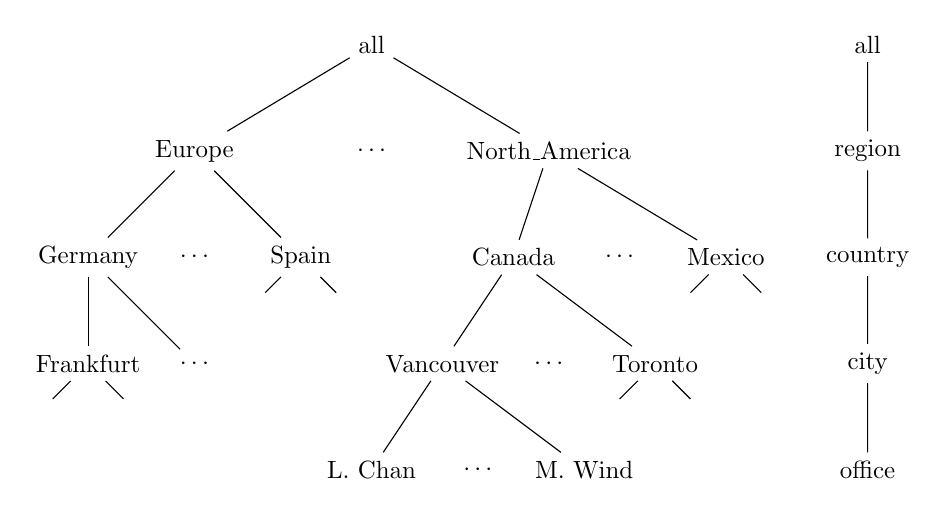
\begin{tikzpicture}[scale=0.9,every node/.style={transform shape}]
		\node at (2,6) (all) {all};

		\node at (-0.5,4.5) (europe) {Europe};
		\node at (2,4.5) (dot1) {$\cdots$};
		\node at (4.5,4.5) (america) {North\_America};

		\node at (-2,3) (germany) {Germany};
		\node at (-0.5,3) (dots2) {$\cdots$};
		\node at (1,3) (spain) {Spain};
		\node at (4,3) (canada) {Canada};
		\node at (5.5,3) (dots3) {$\cdots$};
		\node at (7,3) (mexico) {Mexico};

		\node at (-2,1.5) (frankfurt) {Frankfurt};
		\node at (-0.5,1.5) (dots4) {$\cdots$};
		\node at (3,1.5) (vancouver) {Vancouver};
		\node at (4.5,1.5) (dots5) {$\cdots$};
		\node at (6,1.5) (toronto) {Toronto};
		\node at (2,0) (lchan) {L. Chan};
		\node at (3.5,0) (dots6) {$\cdots$};
		\node at (5,0) (mwind) {M. Wind};

		\draw (all) -- (europe);
		\draw (all) -- (america);
		\draw (europe) -- (germany);
		\draw (europe) -- (spain);
		\draw (america) -- (canada);
		\draw (america) -- (mexico);
		\draw (germany) -- (frankfurt);
		\draw (germany) -- (dots4);
		\draw (spain) -- (0.5,2.5);
		\draw (spain) -- (1.5,2.5);
		\draw (mexico) -- (6.5,2.5);
		\draw (mexico) -- (7.5,2.5);
		\draw (frankfurt) -- (-2.5,1);
		\draw (frankfurt) -- (-1.5,1);
		\draw (toronto) -- (5.5,1);
		\draw (toronto) -- (6.5,1);
		\draw (canada) -- (vancouver);
		\draw (canada) -- (toronto);
		\draw (vancouver) -- (lchan);
		\draw (vancouver) -- (mwind);

		\node at (9,6) (all2) {all};
		\node at (9,4.5) (region2)  {region};
		\node at (9,3) (country2) {country};
		\node at (9,1.5) (city2) {city};
		\node at (9,0) (office2) {office};
		\draw (all2) -- (region2);
		\draw (region2) -- (country2);
		\draw (country2) -- (city2);
		\draw (city2) -- (office2);
	\end{tikzpicture}
\end{frame}

\begin{frame}{Data-Cube Measures: Three Categories}
	\begin{enumerate}
		\item \textbf{Distributive:}
		      \begin{itemize}
			      \item If the result derived by applying the function to the $n$ aggregate values obtained for $n$ partitions of the dataset is the same as that derived by applying the function on all the data without partitioning.\\
			            E.g. \texttt{COUNT, SUM, MIN, MAX}.
		      \end{itemize}
		\item \textbf{Algebraic:}
		      \begin{itemize}
			      \item If it can be computed by an algebraic function with $M$ arguments, each of which is obtained by applying a distributive aggregate function.\\
			            E.g. \texttt{AVG, MIN$_N$, STD}.
		      \end{itemize}
		\item \textbf{Holistic:}
		      \begin{itemize}
			      \item If there is no constant bound on the storage size needed to describe a subaggregate.\\
			            E.g. \texttt{MEDIAN, MODE, RANK}.
		      \end{itemize}
	\end{enumerate}
\end{frame}

\begin{frame}{Aggregation Type}
	\begin{itemize}
		\item \textbf{Non-trivial property.}
		      \begin{itemize}
			      \item Next to name and value range.
		      \end{itemize}
		\item \textbf{Defines the set of aggregation operations that can be executed on a measure (a fact).}
		\item \textbf{\color{airforceblue}FLOW:}
		      \begin{itemize}
			      \item Any aggregation.
			      \item E.g. sales turnover.
		      \end{itemize}
		\item \textbf{\color{airforceblue}STOCK:}
		      \begin{itemize}
			      \item No temporal aggregation.
			      \item E.g. stock, inventory.
		      \end{itemize}
		\item \textbf{\color{airforceblue}VPU (Value per Unit):}
		      \begin{itemize}
			      \item No summarization.
			      \item E.g. price, tax, in general factors.
		      \end{itemize}
		\item \textbf{(Always applicable: \texttt{MIN}, \texttt{MAX} and \texttt{AVG}).}
	\end{itemize}
\end{frame}

\begin{frame}{Aggregation Type}
	\begin{itemize}
		\item \textbf{Sales volume as a function of product, month, and region.}
		      \begin{itemize}
			      \item Dimensions: \texttt{Product, Location, Time.}
			      \item Hierarchical summarization paths.
		      \end{itemize}
	\end{itemize}
	\vspace{0.5cm}
	\hspace{0.5cm}
	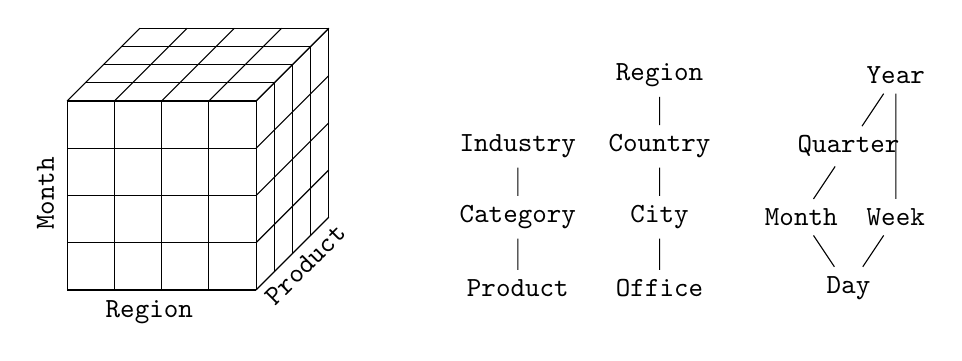
\begin{tikzpicture}[scale=0.6]
		\foreach \x in{0,...,4}
			{   \draw (0,\x ,4) -- (4,\x ,4);
				\draw (\x ,0,4) -- (\x ,4,4);
				\draw (4,\x ,4) -- (4,\x ,0);
				\draw (\x ,4,4) -- (\x ,4,0);
				\draw (4,0,\x ) -- (4,4,\x );
				\draw (0,4,\x ) -- (4,4,\x );
			}

		\node at (0.2,-2) {\texttt{Region}};
		\node[rotate=45] at (3.5,-1) {\texttt{Product}};
		\node[rotate=90] at (-2,0.5) {\texttt{Month}};

		\node at (8,1.5) (industry) {\texttt{Industry}};
		\node at (8,0) (category) {\texttt{Category}};
		\node at (8,-1.5) (product) {\texttt{Product}};
		\draw (industry) -- (category) -- (product);

		\node at (11,3) (region) {\texttt{Region}};
		\node at (11,1.5) (country) {\texttt{Country}};
		\node at (11,0) (city) {\texttt{City}};
		\node at (11,-1.5) (office) {\texttt{Office}};
		\draw (region) -- (country) -- (city) -- (office);

		\node at (16,3) (year) {\texttt{Year}};
		\node at (15,1.5) (quarter) {\texttt{Quarter}};
		\node at (14,0) (month) {\texttt{Month}};
		\node at (16,0) (week) {\texttt{Week}};
		\node at (15,-1.5) (day) {\texttt{Day}};
		\draw (year) -- (quarter) -- (month) -- (day) -- (week) -- (year);
	\end{tikzpicture}
\end{frame}

\begin{frame}{Data Cube Sample}
	\centering
	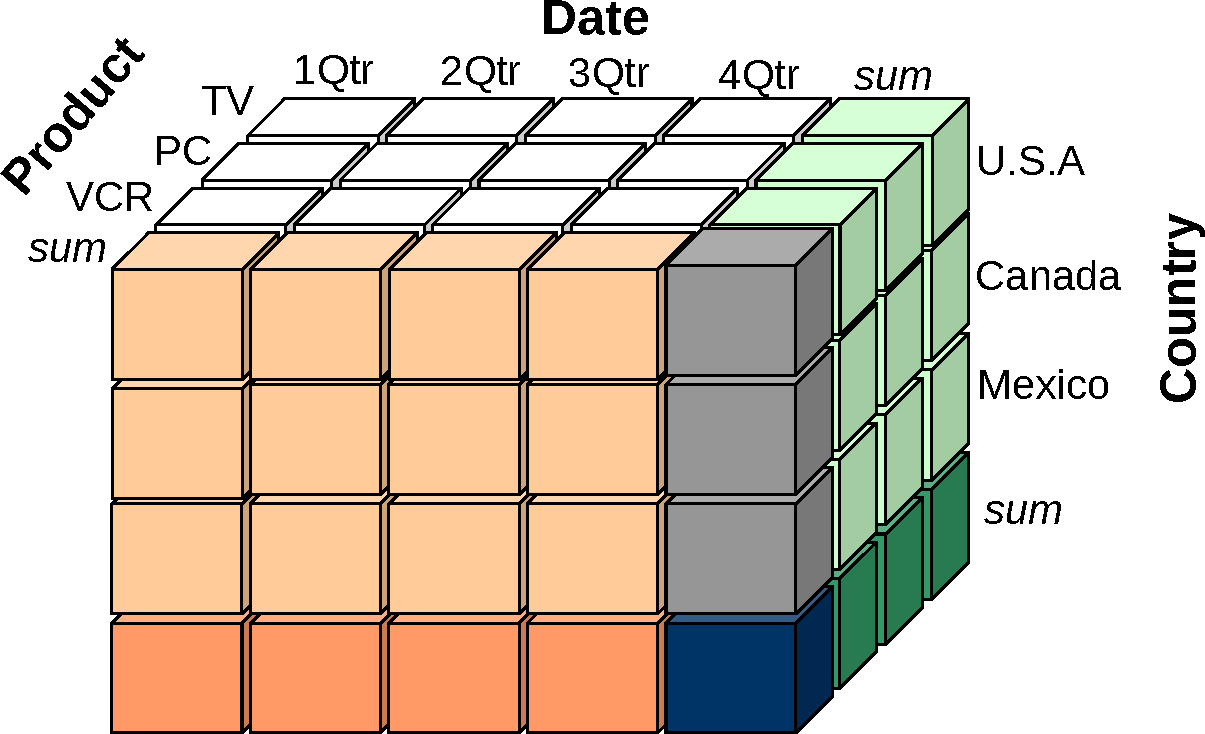
\includegraphics[width=10cm,height=6cm]{img/datacube.pdf}
\end{frame}

\begin{frame}{Cuboids Corresponding to the Cube}
	\centering
	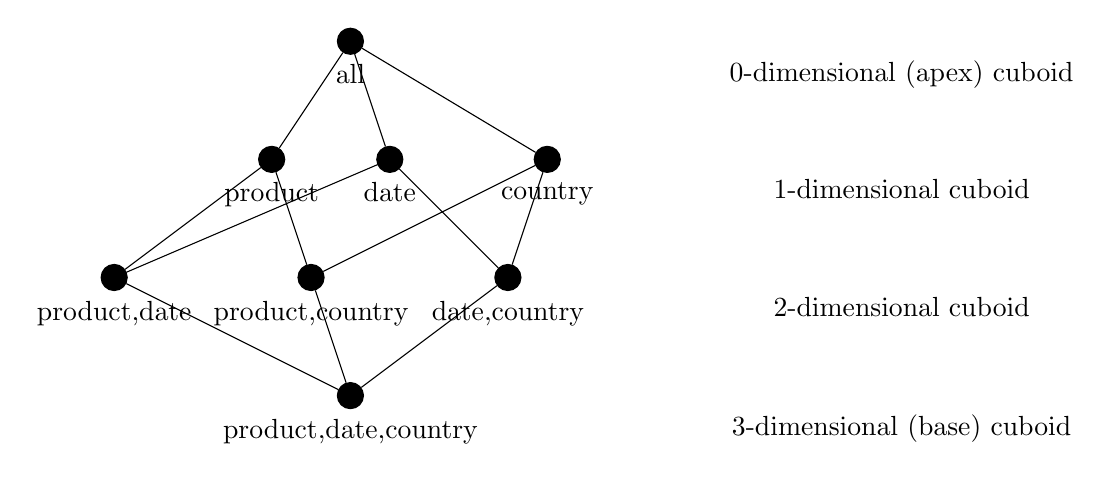
\begin{tikzpicture}
		\node[draw, circle, fill=black, label=below:{all}] at (2,6) (all) {};

		\node[draw, circle, fill=black, label=below:{product}] at (1,4.5) (product) {};
		\node[draw, circle, fill=black, label=below:{date}] at (2.5,4.5) (date) {};
		\node[draw, circle, fill=black, label=below:{country}] at (4.5,4.5) (country) {};

		\node[draw, circle, fill=black, label=below:{product,date}] at (-1,3) (productdate) {};
		\node[draw, circle, fill=black, label=below:{product,country}] at (1.5,3) (productcountry) {};
		\node[draw, circle, fill=black, label=below:{date,country}] at (4,3) (datecountry) {};

		\node[draw, circle, fill=black, label=below:{product,date,country}] at (2,1.5) (productdatecountry) {};

		\node[label=below:{$0$-dimensional (apex) cuboid}] at (9,6)  {};
		\node[label=below:{$1$-dimensional cuboid}] at (9,4.5)  {};
		\node[label=below:{$2$-dimensional cuboid}] at (9,3)  {};
		\node[label=below:{$3$-dimensional (base) cuboid}] at (9,1.5)  {};

		\draw (all) -- (product);
		\draw (all) -- (date);
		\draw (all) -- (country);
		\draw (product) -- (productdate);
		\draw (product) -- (productcountry);
		\draw (date) -- (productdate);
		\draw (date) -- (datecountry);
		\draw (country) -- (productcountry);
		\draw (country) -- (datecountry);
		\draw (productdate) -- (productdatecountry);
		\draw (productcountry) -- (productdatecountry);
		\draw (datecountry) -- (productdatecountry);
	\end{tikzpicture}
\end{frame}

\begin{frame}{Typical OLAP Operations}
	\begin{itemize}
		\item \textbf{{\color{airforceblue}Roll up} (drill up): summarize data.}
		      \begin{itemize}
			      \item By climbing up hierarchy or by dimension reduction.
		      \end{itemize}
		\item \textbf{{\color{airforceblue}Drill down} (roll down): reverse of roll up.}
		      \begin{itemize}
			      \item From higher-level summary to lower-level summary or detailed data, or introducing new dimensions.
		      \end{itemize}
		\item \textbf{{\color{airforceblue}Slice and dice}: project and select.}
		\item \textbf{{\color{airforceblue}Pivot} (rotate):}
		      \begin{itemize}
			      \item Reorient the cube, visualization, 3D to series of 2D planes.
		      \end{itemize}
		\item \textbf{Other operations:}
		      \begin{itemize}
			      \item \textbf{{\color{airforceblue}Drill across}:} involving (across) more than one fact table.
			      \item \textbf{{\color{airforceblue}Drill through}:} through the bottom level of the cube \\ to its back-end relational tables (using SQL).
		      \end{itemize}
	\end{itemize}
\end{frame}
